\chapter{Building A Tiny GPT: The First Complete Walkthrough}

This chapter begins the textbook with one concrete sample case. We will build the mental model for a tiny GPT-style language model before studying every part in detail. The goal is not to finish all mathematics in one chapter. The goal is to see the entire system once, from text to training loss to generated text.

\section{Chapter Goals}

By the end of this chapter, you should be able to:

\begin{itemize}
  \item explain the task solved by a GPT-style language model;
  \item trace one sentence through tokenization, tensors, embeddings, logits, and loss;
  \item identify the main components of a training repository;
  \item understand why small GPT models are the right first experiments;
  \item answer basic conceptual questions about next-token prediction.
\end{itemize}

We will use a sample model called \term{TinyGPT}. TinyGPT is not meant to be impressive. It is meant to be understandable. In machine learning, the first correct small system is more valuable than a large system nobody can debug.

\section{The Sample Case}

Suppose our tiny training corpus contains short sentences about MapleAI and language models:

\begin{lstlisting}
MapleAI trains tiny GPT models.
Tiny GPT models learn from tokens.
Tokens become vectors.
Vectors flow through attention.
\end{lstlisting}

This corpus is too small for a useful real model, but it is perfect for learning. We can see every step without being buried under billions of tokens.

Our first model will learn the following task:

\begin{quote}
Given the tokens so far, predict the next token.
\end{quote}

This is called \term{next-token prediction}. If the context is

\begin{quote}
\texttt{Tiny GPT models learn from}
\end{quote}

then a model trained on the sample corpus should place high probability on the next token \texttt{tokens}. It may also assign some probability to other tokens, but the correct next token in this training example is \texttt{tokens}.

\section{What Is A GPT Model?}

GPT stands for \term{Generative Pretrained Transformer}.

\begin{longtable}{p{0.24\textwidth}p{0.62\textwidth}}
\toprule
\term{Word} & \term{Meaning in this book} \\
\midrule
Generative & The model can produce new token sequences one token at a time. \\
Pretrained & The model first learns from a broad text corpus using next-token prediction. \\
Transformer & The model architecture is built from attention and feed-forward blocks. \\
\bottomrule
\end{longtable}

A GPT model is \term{autoregressive}. This means it generates text from left to right. At step \(t\), it uses the previous tokens
\[
x_1, x_2, \ldots, x_t
\]
to estimate a probability distribution for the next token:
\[
P(x_{t+1} \mid x_1, x_2, \ldots, x_t).
\]

For the sample sentence, the abstract symbols map to real data like this:

\begin{center}
\begin{tikzpicture}[
  token/.style={draw, rounded corners=2pt, minimum width=1.55cm, minimum height=0.72cm, align=center},
  lab/.style={font=\small},
  arrow/.style={-{Latex[length=2mm]}, thick}
]
\node[token, fill=blue!6] (x1) at (0,0) {\texttt{Tiny}\\{\scriptsize \(x_1\)}};
\node[token, fill=blue!6] (x2) at (1.8,0) {\texttt{GPT}\\{\scriptsize \(x_2\)}};
\node[token, fill=blue!6] (x3) at (3.6,0) {\texttt{models}\\{\scriptsize \(x_3\)}};
\node[token, fill=blue!6] (x4) at (5.4,0) {\texttt{learn}\\{\scriptsize \(x_4\)}};
\node[token, fill=red!8] (target) at (7.2,0) {\texttt{from}\\{\scriptsize \(x_5\)}};
\node[lab] at (2.7,0.95) {known context};
\node[lab, text=maplered] at (7.2,0.95) {next token to predict};
\draw[arrow] (x1.north) .. controls (2.2,1.45) and (5.7,1.45) .. (target.north);
\end{tikzpicture}
\end{center}

In this example,
\[
P(x_5 \mid x_1,x_2,x_3,x_4)
= P(\texttt{from} \mid \texttt{Tiny},\texttt{GPT},\texttt{models},\texttt{learn}).
\]
This is the same formula, but now every symbol points to a real token.

The model is not given the future token while making the prediction. During training, we know the correct next token and use it to compute loss. During generation, we choose a next token from the model's predicted distribution and append it to the context.

\section{The Full Pipeline In One Picture}

\begin{center}
\begin{tikzpicture}[
  node distance=0.7cm,
  box/.style={draw, rounded corners=2pt, minimum height=0.8cm, text width=3.0cm, align=center},
  arrow/.style={-{Latex[length=2.2mm]}, thick}
]
\node[box] (text) {Raw text};
\node[box, right=of text] (tok) {Tokenizer};
\node[box, right=of tok] (ids) {Token IDs};
\node[box, below=of ids] (tensor) {Input/target tensors};
\node[box, left=of tensor] (model) {TinyGPT};
\node[box, left=of model] (logits) {Logits};
\node[box, below=of logits] (loss) {Loss};
\node[box, right=of loss] (grad) {Gradients};
\node[box, right=of grad] (opt) {Optimizer step};
\draw[arrow] (text) -- (tok);
\draw[arrow] (tok) -- (ids);
\draw[arrow] (ids) -- (tensor);
\draw[arrow] (tensor) -- (model);
\draw[arrow] (model) -- (logits);
\draw[arrow] (logits) -- (loss);
\draw[arrow] (loss) -- (grad);
\draw[arrow] (grad) -- (opt);
\draw[arrow] (opt.east) -- ++(0.4,0) |- (model.south);
\end{tikzpicture}
\end{center}

The same pipeline appears in every serious GPT training system:

\begin{lstlisting}
text -> tokenizer -> token ids -> tensors -> model
     -> logits -> loss -> gradients -> optimizer
     -> checkpoint -> sampling
\end{lstlisting}

The same pipeline also appears in source code. The table below is the first bridge between the mathematical idea, the TinyGPT data, and the software function that usually implements it.

\begin{longtable}{p{0.2\textwidth}p{0.25\textwidth}p{0.33\textwidth}}
\toprule
\term{Math idea} & \term{TinyGPT case} & \term{Code responsibility} \\
\midrule
Sequence \(x_1,\ldots,x_t\) & \texttt{Tiny GPT models learn} & store token IDs in a tensor \shape{[B,T]} \\
Vocabulary size \(V\) & 9 known tokens & tokenizer owns \texttt{vocab\_size} \\
Embedding matrix \(E\) & row 2 represents \texttt{Tiny} & \texttt{Embedding(V, C)} lookup \\
Model \(f_\theta(x)\) & TinyGPT forward pass & \texttt{model(x)} returns logits \\
Logits \(z\) & 9 scores for next token & final linear layer maps \(C \rightarrow V\) \\
Probability \(p_i\) & probability of \texttt{tokens} & softmax inside cross entropy or sampler \\
Loss \(-\log p_y\) & penalty for correct ID 7 & \texttt{cross\_entropy(logits, targets)} \\
Gradient \(\nabla_\theta L\) & parameter blame signal & \texttt{loss.backward()} \\
\bottomrule
\end{longtable}

The rest of the book explains each arrow carefully.

\section{Who Does What In A GPT Training System?}

It is helpful to treat TinyGPT training as a small factory. Each part has a job, an input, an output, and a failure mode. The mathematics is not separate from the software: the math defines the contract that each software part must satisfy.

\begin{center}
\begin{tikzpicture}[
  box/.style={draw, rounded corners=2pt, minimum height=0.72cm, text width=2.35cm, align=center},
  arrow/.style={-{Latex[length=2mm]}, thick},
  lab/.style={font=\small, align=center}
]
\node[box, fill=blue!5] (human) at (0,0) {human/data curator\\chooses corpus};
\node[box, fill=blue!5] (prep) at (3.0,0) {data script\\cleans text};
\node[box, fill=blue!5] (tok) at (6.0,0) {tokenizer\\creates IDs};
\node[box, fill=red!8] (loader) at (9.0,0) {data loader\\builds \(x,y\)};
\node[box, fill=red!8] (model) at (9.0,-1.45) {model\\computes logits};
\node[box, fill=red!8] (loss) at (6.0,-1.45) {loss function\\scores mistakes};
\node[box, fill=gray!12] (opt) at (3.0,-1.45) {optimizer\\updates weights};
\node[box, fill=gray!12] (ckpt) at (0,-1.45) {checkpoint\\stores state};
\draw[arrow] (human) -- (prep);
\draw[arrow] (prep) -- (tok);
\draw[arrow] (tok) -- (loader);
\draw[arrow] (loader) -- (model);
\draw[arrow] (model) -- (loss);
\draw[arrow] (loss) -- (opt);
\draw[arrow] (opt) -- (ckpt);
\draw[arrow] (opt.north) .. controls (5.0,-0.7) and (7.8,-0.85) .. (model.west);
\node[lab] at (4.7,-2.35) {Training is a loop: data creates predictions, loss creates gradients, optimizer changes parameters.};
\end{tikzpicture}
\end{center}

\begin{longtable}{p{0.18\textwidth}p{0.24\textwidth}p{0.24\textwidth}p{0.22\textwidth}}
\toprule
\term{Part} & \term{Receives} & \term{Produces} & \term{Main risk} \\
\midrule
Data curator & raw documents & approved corpus & bad or unsafe data \\
Tokenizer & text & token IDs & inconsistent vocabulary \\
Data loader & token stream & \(x,y\) batches & off-by-one target shift \\
Model & \(x\) & logits \(Z\) & wrong shapes or mask \\
Loss & logits and \(y\) & scalar \(L\) & wrong target alignment \\
Optimizer & gradients & new parameters & unstable learning rate \\
Checkpoint & states and config & resumable artifact & missing metadata \\
\bottomrule
\end{longtable}

This table is a practical debugging map. If generated text is poor, do not only blame the model. Check the whole chain: data, tokenizer, target shift, shapes, loss, optimizer, and checkpoint loading.

\section{The Four Views Of One Training Example}

The same TinyGPT example can be seen in four synchronized views.

\begin{center}
\begin{tikzpicture}[
  box/.style={draw, rounded corners=2pt, minimum height=0.85cm, text width=2.65cm, align=center},
  arrow/.style={-{Latex[length=2mm]}, thick}
]
\node[box, fill=blue!5] (real) at (0,0) {real text\\\texttt{Tiny GPT models learn}};
\node[box, fill=blue!5] (data) at (3.1,0) {data view\\\([2,3,4,5]\)};
\node[box, fill=red!8] (math) at (6.2,0) {math view\\\(x\in\mathbb{Z}^{1\times4}\)};
\node[box, fill=red!8] (model) at (9.3,0) {model view\\logits \shape{[1,4,9]}};
\node[box, fill=gray!12] (result) at (9.3,-1.55) {result view\\loss and sample};
\draw[arrow] (real) -- (data);
\draw[arrow] (data) -- (math);
\draw[arrow] (math) -- (model);
\draw[arrow] (model) -- (result);
\end{tikzpicture}
\end{center}

These views answer different questions:

\begin{itemize}
  \item The real-text view asks, ``What sentence are we teaching from?''
  \item The data view asks, ``What exact IDs enter the program?''
  \item The math view asks, ``What object and shape does the equation describe?''
  \item The model view asks, ``What tensor does the neural network produce?''
  \item The result view asks, ``Did the model assign probability to the correct next token?''
\end{itemize}

For a beginner, many GPT mistakes happen because these views become disconnected. A professional training workflow keeps them aligned.

\section{One Prediction, End To End}

The next diagram follows one supervised prediction through the whole system. The model sees the context ending in \texttt{from}; the target is \texttt{tokens}. This is the most important mental picture in the book.

\begin{center}
\begin{tikzpicture}[
  token/.style={draw, minimum width=1.15cm, minimum height=0.58cm, align=center},
  box/.style={draw, rounded corners=2pt, minimum height=0.72cm, text width=2.25cm, align=center},
  arrow/.style={-{Latex[length=2mm]}, thick},
  lab/.style={font=\small, align=center}
]
\node[lab] at (2.0,1.0) {visible context \(x\)};
\foreach \i/\tok/\id in {0/Tiny/2,1/GPT/3,2/models/4,3/learn/5,4/from/6} {
  \node[token, fill=blue!5] (t\i) at (\i*1.15,0) {\texttt{\tok}\\{\scriptsize ID \id}};
}
\node[token, fill=red!10] (target) at (6.7,0) {\texttt{tokens}\\{\scriptsize target ID 7}};
\draw[arrow] (5.1,0) -- (target);
\node[box, fill=blue!5] (embed) at (1.8,-1.35) {embedding lookup\\\shape{[1,5,6]}};
\node[box, fill=blue!5] (block) at (4.6,-1.35) {TinyGPT blocks\\context mixing};
\node[box, fill=red!8] (logits) at (7.4,-1.35) {last-position logits\\\shape{[9]}};
\node[box, fill=red!8] (loss) at (7.4,-2.85) {loss\\\(-\log p_7\)};
\node[box, fill=gray!12] (update) at (4.6,-2.85) {optimizer\\updates \(\theta\)};
\draw[arrow] (t2.south) -- (embed.north);
\draw[arrow] (embed) -- (block);
\draw[arrow] (block) -- (logits);
\draw[arrow] (logits) -- (loss);
\draw[arrow] (loss) -- (update);
\draw[arrow] (update.west) .. controls (2.7,-2.9) and (2.4,-2.0) .. (block.south);
\node[lab] at (1.4,-2.65) {data loader owns \(x,y\)};
\node[lab] at (9.65,-2.15) {loss checks whether\\ID 7 got high probability};
\end{tikzpicture}
\end{center}

The flow has five different kinds of objects:

\begin{longtable}{p{0.18\textwidth}p{0.26\textwidth}p{0.38\textwidth}}
\toprule
\term{Object} & \term{Example} & \term{Who manages it} \\
\midrule
Text & \texttt{Tiny GPT models learn from} & dataset and tokenizer code \\
IDs & \([2,3,4,5,6]\) & data loader \\
Vectors & \shape{[1,5,6]} & model embedding layer \\
Scores & logits \shape{[9]} & output head \\
Result & loss scalar & loss function and trainer \\
\bottomrule
\end{longtable}

This diagram is also the debugging order. If the result is wrong, inspect the IDs before the embeddings, inspect the embeddings before the logits, and inspect the logits before blaming the optimizer.

\section{Step 1: Raw Text}

The starting point is ordinary text:

\begin{quote}
\texttt{Tiny GPT models learn from tokens.}
\end{quote}

Text is easy for humans to read, but a neural network does not process words directly. Neural networks process arrays of numbers. Therefore, the first engineering problem is to convert text into numerical IDs.

\section{Step 2: Tokenization}

A \term{tokenizer} converts text into tokens. In a real GPT system, tokens may be words, word pieces, bytes, punctuation marks, or common character sequences. For this first chapter, use a simple word-level tokenizer so the idea is visible.

Assume the tokenizer learns this tiny vocabulary:

\begin{longtable}{p{0.24\textwidth}p{0.24\textwidth}p{0.34\textwidth}}
\toprule
\term{Token} & \term{ID} & \term{Comment} \\
\midrule
\texttt{MapleAI} & 0 & organization token \\
\texttt{trains} & 1 & verb \\
\texttt{Tiny} & 2 & adjective \\
\texttt{GPT} & 3 & model family token \\
\texttt{models} & 4 & noun \\
\texttt{learn} & 5 & verb \\
\texttt{from} & 6 & preposition \\
\texttt{tokens} & 7 & noun \\
\texttt{.} & 8 & punctuation \\
\bottomrule
\end{longtable}

Then the sentence

\begin{quote}
\texttt{Tiny GPT models learn from tokens .}
\end{quote}

might become:

\[
[2, 3, 4, 5, 6, 7, 8].
\]

The mapping can be drawn as a two-row strip:

\begin{center}
\begin{tikzpicture}[
  cell/.style={draw, minimum width=1.6cm, minimum height=0.7cm, align=center},
  idcell/.style={draw, minimum width=1.6cm, minimum height=0.55cm, align=center, fill=blue!5},
  arrow/.style={-{Latex[length=2mm]}, thick}
]
\node[cell] (t1) at (0,0) {\texttt{Tiny}};
\node[cell] (t2) at (1.65,0) {\texttt{GPT}};
\node[cell] (t3) at (3.3,0) {\texttt{models}};
\node[cell] (t4) at (4.95,0) {\texttt{learn}};
\node[cell] (t5) at (6.6,0) {\texttt{from}};
\node[cell] (t6) at (8.25,0) {\texttt{tokens}};
\node[cell] (t7) at (9.9,0) {\texttt{.}};
\node[idcell] at (0,-0.85) {2};
\node[idcell] at (1.65,-0.85) {3};
\node[idcell] at (3.3,-0.85) {4};
\node[idcell] at (4.95,-0.85) {5};
\node[idcell] at (6.6,-0.85) {6};
\node[idcell] at (8.25,-0.85) {7};
\node[idcell] at (9.9,-0.85) {8};
\node[align=right] at (-1.35,0) {\small tokens};
\node[align=right] at (-1.35,-0.85) {\small ids};
\foreach \x in {0,1.65,3.3,4.95,6.6,8.25,9.9}
  \draw[arrow] (\x,-0.25) -- (\x,-0.58);
\end{tikzpicture}
\end{center}

The exact token IDs are not meaningful by themselves. Token ID \(7\) is not mathematically ``larger'' than token ID \(3\) in a language sense. The ID is an index into a learned embedding table.

\section{Step 3: Input And Target Sequences}

GPT training uses shifted sequences. If the token stream is
\[
[2, 3, 4, 5, 6, 7, 8],
\]
and the context length is \(T=4\), then one training example can be:

\[
x = [2, 3, 4, 5],
\]
\[
y = [3, 4, 5, 6].
\]

The input \(x\) asks the model to predict:

\begin{longtable}{p{0.28\textwidth}p{0.28\textwidth}p{0.28\textwidth}}
\toprule
\term{Position} & \term{Context token} & \term{Target next token} \\
\midrule
0 & \texttt{Tiny} & \texttt{GPT} \\
1 & \texttt{GPT} & \texttt{models} \\
2 & \texttt{models} & \texttt{learn} \\
3 & \texttt{learn} & \texttt{from} \\
\bottomrule
\end{longtable}

This is the first essential GPT pattern:

\begin{lstlisting}
input:  token 0, token 1, token 2, token 3
target: token 1, token 2, token 3, token 4
\end{lstlisting}

Every target is the next token after the matching input position.

The shift is easier to see as parallel tracks:

\begin{center}
\begin{tikzpicture}[
  cell/.style={draw, minimum width=1.55cm, minimum height=0.62cm, align=center},
  incell/.style={cell, fill=blue!5},
  outcell/.style={cell, fill=red!6},
  lab/.style={font=\small},
  arrow/.style={-{Latex[length=2mm]}, thick}
]
\node[lab] at (-1.2,0) {input \(x\)};
\node[incell] (x0) at (0,0) {2\\{\scriptsize Tiny}};
\node[incell] (x1) at (1.7,0) {3\\{\scriptsize GPT}};
\node[incell] (x2) at (3.4,0) {4\\{\scriptsize models}};
\node[incell] (x3) at (5.1,0) {5\\{\scriptsize learn}};
\node[lab] at (-1.2,-1.25) {target \(y\)};
\node[outcell] (y0) at (0,-1.25) {3\\{\scriptsize GPT}};
\node[outcell] (y1) at (1.7,-1.25) {4\\{\scriptsize models}};
\node[outcell] (y2) at (3.4,-1.25) {5\\{\scriptsize learn}};
\node[outcell] (y3) at (5.1,-1.25) {6\\{\scriptsize from}};
\foreach \a/\b in {x0/y0,x1/y1,x2/y2,x3/y3}
  \draw[arrow] (\a.south) -- (\b.north);
\node[align=left, font=\small] at (8.1,-0.62) {Each column is one\\supervised prediction.};
\end{tikzpicture}
\end{center}

So the mathematical pair
\[
(x_t,y_t)=(x_t,x_{t+1})
\]
means something very concrete: the token currently visible at a position is used to predict the token immediately after it.

\section{Step 4: Tensors And Shapes}

Training uses batches. If batch size is \(B=2\) and context length is \(T=4\), the input tensor has shape
\[
x \in \mathbb{Z}^{2 \times 4}.
\]
For example:

\[
x =
\begin{bmatrix}
2 & 3 & 4 & 5 \\
0 & 1 & 2 & 3
\end{bmatrix},
\qquad
y =
\begin{bmatrix}
3 & 4 & 5 & 6 \\
1 & 2 & 3 & 4
\end{bmatrix}.
\]

The shape \shape{[B, T]} means:

\begin{itemize}
  \item \(B\): how many sequences are processed together;
  \item \(T\): how many token positions are in each sequence.
\end{itemize}

Shape reasoning is one of the most important practical skills in LLM training. If the shape is wrong, the mathematics is usually wrong too.

The batch can be read as a small spreadsheet of token IDs:

\begin{center}
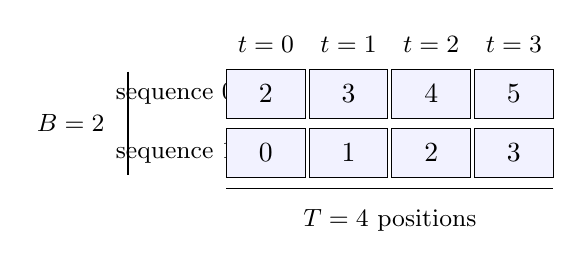
\begin{tikzpicture}[
  cell/.style={draw, minimum width=1.0cm, minimum height=0.62cm, align=center},
  rowlab/.style={font=\small, align=right},
  collab/.style={font=\small}
]
\node[rowlab] at (-1.15,0) {sequence 0};
\node[rowlab] at (-1.15,-0.75) {sequence 1};
\foreach \i/\v in {0/2,1/3,2/4,3/5}
  \node[cell, fill=blue!5] at (\i*1.05,0) {\v};
\foreach \i/\v in {0/0,1/1,2/2,3/3}
  \node[cell, fill=blue!5] at (\i*1.05,-0.75) {\v};
\foreach \i in {0,1,2,3}
  \node[collab] at (\i*1.05,0.62) {\(t=\i\)};
\draw[decorate] (-0.5,-1.2) -- node[below=4pt] {\small \(T=4\) positions} (3.65,-1.2);
\draw[decorate] (-1.75,0.28) -- node[left=5pt] {\small \(B=2\)} (-1.75,-1.03);
\end{tikzpicture}
\end{center}

The notation \(x \in \mathbb{Z}^{2 \times 4}\) is just the mathematical way of saying ``two rows, four token IDs per row.''

\section{Step 5: Embeddings}

Token IDs are indices. The model must convert them into vectors. If the vocabulary size is \(V=9\) and the embedding dimension is \(C=6\), then the token embedding table has shape
\[
E_{\text{tok}} \in \mathbb{R}^{9 \times 6}.
\]

Each token ID selects one row. After embedding, the tensor shape changes:

\[
\shape{[B, T]} \rightarrow \shape{[B, T, C]}.
\]

For our sample:

\[
\shape{[2, 4]} \rightarrow \shape{[2, 4, 6]}.
\]

This means each token position is now represented by a vector of six learned numbers. Real GPT models use much larger dimensions, such as 768, 1024, or more.

The embedding lookup is not a calculation like \(2 \times 6\). It is a table lookup:

\begin{center}
\begin{tikzpicture}[
  small/.style={draw, minimum width=0.62cm, minimum height=0.48cm, align=center},
  box/.style={draw, rounded corners=2pt, minimum width=1.2cm, minimum height=0.65cm, align=center},
  arrow/.style={-{Latex[length=2mm]}, thick}
]
\node[box, fill=blue!5] (id) at (0,0) {ID 2};
\node[box] (row) at (2.1,0) {row 2 of \(E_{\text{tok}}\)};
\node[small, fill=red!5] at (4.0,0) {\(e_1\)};
\node[small, fill=red!5] at (4.62,0) {\(e_2\)};
\node[small, fill=red!5] at (5.24,0) {\(e_3\)};
\node[small, fill=red!5] at (5.86,0) {\(e_4\)};
\node[small, fill=red!5] at (6.48,0) {\(e_5\)};
\node[small, fill=red!5] at (7.10,0) {\(e_6\)};
\draw[arrow] (id) -- (row);
\draw[arrow] (row) -- (3.65,0);
\node[font=\small, align=center] at (5.55,-0.75) {six learned numbers because \(C=6\)};
\end{tikzpicture}
\end{center}

After this lookup, token \texttt{Tiny} is no longer just ID \(2\). It is a vector that the model can add, multiply, compare, and update during training.

\section{Step 6: The Transformer}

The Transformer is the main model body. It repeatedly applies two ideas:

\begin{itemize}
  \item \term{attention}: each position reads information from previous positions;
  \item \term{feed-forward transformation}: each position's vector is transformed through learned linear layers and nonlinearities.
\end{itemize}

A causal GPT model can use tokens on the left, but not tokens on the right. When predicting the token after \texttt{models}, the model can use:

\begin{quote}
\texttt{Tiny GPT models}
\end{quote}

but not:

\begin{quote}
\texttt{learn from tokens}
\end{quote}

because those are future tokens relative to that prediction.

For the context \texttt{Tiny GPT models learn}, causal attention allows this reading pattern:

\begin{center}
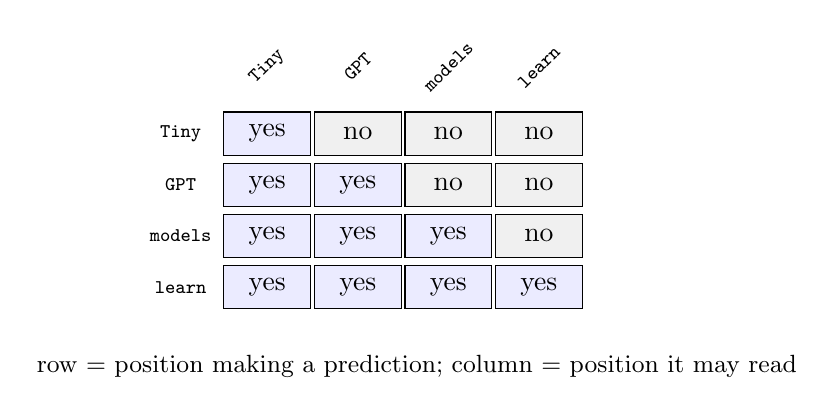
\begin{tikzpicture}[
  cell/.style={draw, minimum width=1.1cm, minimum height=0.55cm, align=center},
  yes/.style={cell, fill=blue!8},
  no/.style={cell, fill=gray!12},
  lab/.style={font=\scriptsize}
]
\foreach \i/\name in {0/Tiny,1/GPT,2/models,3/learn} {
  \node[lab, rotate=45] at (\i*1.15+1.1,0.55) {\texttt{\name}};
  \node[lab] at (0,\i*-0.65-0.3) {\texttt{\name}};
}
\foreach \r in {0,1,2,3} {
  \foreach \c in {0,1,2,3} {
    \ifnum\c>\r
      \node[no] at (\c*1.15+1.1,\r*-0.65-0.3) {no};
    \else
      \node[yes] at (\c*1.15+1.1,\r*-0.65-0.3) {yes};
    \fi
  }
}
\node[font=\small, align=center] at (3.0,-3.25) {row = position making a prediction; column = position it may read};
\end{tikzpicture}
\end{center}

The lower-triangular pattern is the visual form of ``no future tokens.'' This is why GPT can be trained on complete text while still learning a left-to-right generation rule.

\section{Step 7: Logits}

The model outputs \term{logits}. A logit is a raw score before probability normalization. For each position, the model produces one score for every vocabulary token.

If \(B=2\), \(T=4\), and \(V=9\), then logits have shape:

\[
\shape{[2, 4, 9]}.
\]

At each position, the model is saying:

\begin{quote}
Here are my nine scores for the next token.
\end{quote}

Softmax converts those scores into probabilities:

\[
p_i = \frac{e^{z_i}}{\sum_{j=1}^{V} e^{z_j}}.
\]

Here is a concrete example for one position. Suppose the model has seen:

\begin{quote}
\texttt{Tiny GPT models learn from}
\end{quote}

The correct next token is \texttt{tokens}, ID \(7\). TinyGPT produces one logit for every vocabulary token:

\begin{center}
\begin{tikzpicture}[
  bar/.style={draw, fill=blue!12, minimum height=0.45cm},
  targ/.style={draw, fill=red!18, minimum height=0.45cm},
  lab/.style={font=\scriptsize}
]
\node[lab, align=right] at (-1.15,0) {token ID};
\foreach \i/\w/\h in {0/MapleAI/0.4,1/trains/0.6,2/Tiny/0.5,3/GPT/0.7,4/models/0.8,5/learn/0.9,6/from/0.7,7/tokens/2.2,8/./0.3} {
  \node[lab] at (\i*1.0,0) {\i};
  \node[lab, rotate=45, anchor=west] at (\i*1.0,-0.25) {\texttt{\w}};
  \ifnum\i=7
    \node[targ, anchor=south, minimum width=0.5cm, minimum height=\h cm] at (\i*1.0,0.28) {};
  \else
    \node[bar, anchor=south, minimum width=0.5cm, minimum height=\h cm] at (\i*1.0,0.28) {};
  \fi
}
\node[font=\small, text=maplered] at (7,2.85) {largest score};
\end{tikzpicture}
\end{center}

If softmax turns these logits into \(p_{\texttt{tokens}}=0.64\), then the model assigns \(64\%\) probability to the correct next token at this position.

The full shape story from input IDs to logits is:

\begin{center}
\begin{tikzpicture}[
  box/.style={draw, rounded corners=2pt, minimum height=0.75cm, text width=2.4cm, align=center},
  arrow/.style={-{Latex[length=2mm]}, thick},
  note/.style={font=\small, align=center}
]
\node[box, fill=blue!5] (ids) at (0,0) {token IDs\\\shape{[B,T]}};
\node[box, fill=blue!5] (emb) at (3.0,0) {embeddings\\\shape{[B,T,C]}};
\node[box, fill=blue!5] (blocks) at (6.0,0) {Transformer\\\shape{[B,T,C]}};
\node[box, fill=red!8] (logits) at (9.0,0) {logits\\\shape{[B,T,V]}};
\draw[arrow] (ids) -- (emb);
\draw[arrow] (emb) -- (blocks);
\draw[arrow] (blocks) -- (logits);
\node[note] at (1.5,-0.85) {lookup rows};
\node[note] at (4.5,-0.85) {mix context};
\node[note] at (7.5,-0.85) {score vocabulary};
\end{tikzpicture}
\end{center}

For TinyGPT in this chapter, \(B=2\), \(T=4\), \(C=6\), and \(V=9\). Therefore:

\[
\shape{[2,4]} \rightarrow \shape{[2,4,6]} \rightarrow \shape{[2,4,6]} \rightarrow \shape{[2,4,9]}.
\]

The middle shape stays \shape{[B,T,C]} because Transformer blocks change the content of each vector, not the number of sequences, positions, or channels.

\section{Step 8: Loss}

The training loss measures how surprised the model is by the correct next token. If the correct next token is \(y\), and the model assigns probability \(p_y\), then the loss for that prediction is:

\[
\ell = -\log p_y.
\]

If the model assigns high probability to the correct token, the loss is small. If it assigns low probability to the correct token, the loss is large.

For the concrete \texttt{tokens} example:

\[
y = 7,\qquad p_y = p_{\texttt{tokens}} = 0.64.
\]

The loss is:

\[
\ell = -\log(0.64) \approx 0.446.
\]

If the model had assigned only \(p_y=0.05\), the loss would be:

\[
\ell = -\log(0.05) \approx 2.996.
\]

So the loss is not a mysterious score. It is a numerical penalty for not trusting the correct next token enough.

\begin{center}
\begin{tikzpicture}[
  box/.style={draw, rounded corners=2pt, minimum height=0.7cm, text width=2.6cm, align=center},
  arrow/.style={-{Latex[length=2mm]}, thick}
]
\node[box, fill=blue!5] (logits) at (0,0) {logits\\raw scores};
\node[box, fill=blue!5] (softmax) at (3.2,0) {softmax\\probabilities};
\node[box, fill=red!8] (pick) at (6.4,0) {select target\\\(p_y=0.64\)};
\node[box, fill=red!8] (loss) at (9.6,0) {loss\\\(-\log 0.64\)};
\draw[arrow] (logits) -- (softmax);
\draw[arrow] (softmax) -- (pick);
\draw[arrow] (pick) -- (loss);
\end{tikzpicture}
\end{center}

For a batch, the cross-entropy loss averages over all \(B \times T\) predictions:

\[
L = -\frac{1}{BT}\sum_{b=1}^{B}\sum_{t=1}^{T}\log p_{b,t,y_{b,t}}.
\]

\section{Step 9: Gradients And The Optimizer}

The model contains parameters: embedding rows, attention matrices, feed-forward matrices, normalization weights, and output weights. Training means changing those parameters to reduce loss.

Backpropagation computes the gradient:

\[
\nabla_{\theta} L.
\]

The optimizer updates the parameters. A simple gradient descent update is:

\[
\theta_{\text{new}} = \theta_{\text{old}} - \eta \nabla_{\theta}L,
\]

where \(\eta\) is the learning rate. Real training often uses AdamW rather than plain gradient descent, but the principle is the same: use the gradient to change parameters in a direction that tends to reduce loss.

\section{Step 10: Checkpoints And Sampling}

A \term{checkpoint} saves training state. A useful checkpoint includes:

\begin{itemize}
  \item model weights;
  \item optimizer state;
  \item model config;
  \item tokenizer identity;
  \item current training step;
  \item random seed or random number generator states when possible.
\end{itemize}

After training, we can sample from the model. Sampling starts with a prompt:

\begin{quote}
\texttt{Tiny GPT}
\end{quote}

The model predicts a distribution for the next token. We choose one token, append it, and repeat:

\begin{lstlisting}
Tiny GPT
Tiny GPT models
Tiny GPT models learn
Tiny GPT models learn from
Tiny GPT models learn from tokens
\end{lstlisting}

This is generation. It is still next-token prediction, used repeatedly.

\section{TinyGPT Source Code Logic}

Now we connect the same ideas to code. This is not yet a production implementation. It is a readable teaching skeleton. The purpose is to understand how every mathematical object becomes a software object.

\subsection{Code Map}

\begin{center}
\begin{tikzpicture}[
  box/.style={draw, rounded corners=2pt, minimum height=0.75cm, text width=2.65cm, align=center},
  arrow/.style={-{Latex[length=2mm]}, thick}
]
\node[box, fill=blue!5] (tok) at (0,0) {\texttt{encode}\\text to IDs};
\node[box, fill=blue!5] (batch) at (3.0,0) {\texttt{make\_batch}\\IDs to \(x,y\)};
\node[box, fill=blue!5] (forward) at (6.0,0) {\texttt{forward}\\\(x\) to logits};
\node[box, fill=red!8] (loss) at (9.0,0) {\texttt{loss}\\logits vs \(y\)};
\node[box, fill=red!8] (step) at (6.0,-1.35) {\texttt{train\_step}\\update weights};
\node[box, fill=blue!5] (gen) at (3.0,-1.35) {\texttt{generate}\\sample tokens};
\draw[arrow] (tok) -- (batch);
\draw[arrow] (batch) -- (forward);
\draw[arrow] (forward) -- (loss);
\draw[arrow] (loss) |- (step);
\draw[arrow] (step) -- (gen);
\end{tikzpicture}
\end{center}

Read this diagram left to right. The tokenizer prepares numbers. The batch function creates supervised examples. The model forward pass computes logits. The loss compares those logits to targets. The training step updates weights. Generation uses the trained model repeatedly.

\subsection{Tokenizer Functions}

The tokenizer owns the vocabulary. In this first chapter we use a tiny word-level tokenizer:

\begin{lstlisting}[language=Python]
token_to_id = {
    "MapleAI": 0,
    "trains": 1,
    "Tiny": 2,
    "GPT": 3,
    "models": 4,
    "learn": 5,
    "from": 6,
    "tokens": 7,
    ".": 8,
}
id_to_token = {i: tok for tok, i in token_to_id.items()}

def encode(text):
    tokens = text.split()
    return [token_to_id[tok] for tok in tokens]

def decode(ids):
    tokens = [id_to_token[i] for i in ids]
    return " ".join(tokens)
\end{lstlisting}

\term{What the code does}: \texttt{encode()} maps visible text tokens to integer IDs. \texttt{decode()} maps IDs back to text tokens.

\term{How this maps to math}: the vocabulary is the set \(\{0,\ldots,V-1\}\). Here \(V=9\). The token sequence
\[
[\texttt{Tiny},\texttt{GPT},\texttt{models},\texttt{learn},\texttt{from},\texttt{tokens},\texttt{.}]
\]
becomes
\[
[2,3,4,5,6,7,8].
\]

\term{Why it works}: neural networks need numeric inputs. The tokenizer creates a stable contract between text and numbers. If this contract changes, the model weights no longer mean the same thing.

\subsection{Batch Function}

The batch function creates \(x\) and \(y\). The important idea is the one-token shift.

\begin{lstlisting}[language=Python]
def make_one_example(ids, start, block_size):
    chunk = ids[start : start + block_size + 1]
    x = chunk[:-1]
    y = chunk[1:]
    return x, y
\end{lstlisting}

For:

\begin{lstlisting}
ids = [2, 3, 4, 5, 6, 7, 8]
block_size = 4
start = 0
\end{lstlisting}

the chunk is:

\[
[2,3,4,5,6].
\]

Then:

\[
x=[2,3,4,5],
\qquad
y=[3,4,5,6].
\]

\begin{center}
\begin{tikzpicture}[
  cell/.style={draw, minimum width=0.9cm, minimum height=0.55cm, align=center},
  arrow/.style={-{Latex[length=2mm]}, thick},
  lab/.style={font=\small}
]
\foreach \i/\v in {0/2,1/3,2/4,3/5,4/6} {
  \node[cell, fill=gray!8] at (\i*1.0,0) {\v};
}
\node[lab] at (-0.8,0) {chunk};
\foreach \i/\v in {0/2,1/3,2/4,3/5} {
  \node[cell, fill=blue!6] at (\i*1.0,-1.0) {\v};
}
\node[lab] at (-0.8,-1.0) {\(x\)};
\foreach \i/\v in {0/3,1/4,2/5,3/6} {
  \node[cell, fill=red!8] at (\i*1.0,-2.0) {\v};
}
\node[lab] at (-0.8,-2.0) {\(y\)};
\draw[arrow] (0,-0.3) -- (0,-0.72);
\draw[arrow] (1,-0.3) -- (0,-1.72);
\node[lab, align=left] at (5.7,-1.0) {same chunk\\two shifted views};
\end{tikzpicture}
\end{center}

\term{Why the function needs \texttt{block\_size + 1}}: to build \(T\) input tokens and \(T\) target tokens, the loader needs one extra future token. Without the extra token, the final input position would not have a target.

\subsection{Model Configuration}

A model config records the sizes that appear in the math:

\begin{lstlisting}[language=Python]
config = {
    "vocab_size": 9,    # V
    "block_size": 4,    # T
    "n_embd": 6,        # C
    "n_layer": 2,
    "n_head": 2,
}
\end{lstlisting}

This tiny config means:

\begin{longtable}{p{0.22\textwidth}p{0.2\textwidth}p{0.42\textwidth}}
\toprule
\term{Config} & \term{Symbol} & \term{Meaning} \\
\midrule
\texttt{vocab\_size} & \(V=9\) & nine possible next-token classes \\
\texttt{block\_size} & \(T=4\) & four context positions per example \\
\texttt{n\_embd} & \(C=6\) & each token becomes a six-number vector \\
\texttt{n\_layer} & 2 & two Transformer blocks \\
\texttt{n\_head} & 2 & two attention heads per block \\
\bottomrule
\end{longtable}

\term{Why config matters}: source code should not hide model dimensions. If the checkpoint says the output head has shape \(6 \times 9\), the config must explain that \(C=6\) and \(V=9\).

\subsection{The TinyGPT Module}

A GPT model is a function with parameters:

\[
f_\theta(x) = \text{logits}.
\]

In PyTorch-style code, that idea becomes a class:

\begin{lstlisting}[language=Python]
class TinyGPT(nn.Module):
    def __init__(self, config):
        super().__init__()
        V = config["vocab_size"]
        T = config["block_size"]
        C = config["n_embd"]

        self.token_emb = nn.Embedding(V, C)
        self.pos_emb = nn.Embedding(T, C)
        self.blocks = nn.ModuleList([
            TransformerBlock(config)
            for _ in range(config["n_layer"])
        ])
        self.ln_f = nn.LayerNorm(C)
        self.lm_head = nn.Linear(C, V)
\end{lstlisting}

\term{Block by block}:

\begin{itemize}
  \item \texttt{token\_emb}: maps token IDs to vectors, \(V \rightarrow C\).
  \item \texttt{pos\_emb}: gives each position \(0,\ldots,T-1\) its own vector.
  \item \texttt{blocks}: repeated Transformer blocks that mix context.
  \item \texttt{ln\_f}: final normalization for stable hidden states.
  \item \texttt{lm\_head}: maps each hidden vector back to \(V\) logits.
\end{itemize}

Visually:

\begin{center}
\begin{tikzpicture}[
  box/.style={draw, rounded corners=2pt, minimum height=0.75cm, text width=2.25cm, align=center},
  arrow/.style={-{Latex[length=2mm]}, thick}
]
\node[box, fill=blue!5] (id) at (0,0) {IDs\\\shape{[B,T]}};
\node[box, fill=blue!5] (emb) at (2.7,0) {token + pos\\\shape{[B,T,C]}};
\node[box, fill=blue!5] (blk) at (5.4,0) {blocks\\\shape{[B,T,C]}};
\node[box, fill=blue!5] (ln) at (8.1,0) {LayerNorm\\\shape{[B,T,C]}};
\node[box, fill=red!8] (head) at (10.8,0) {head\\\shape{[B,T,V]}};
\draw[arrow] (id) -- (emb);
\draw[arrow] (emb) -- (blk);
\draw[arrow] (blk) -- (ln);
\draw[arrow] (ln) -- (head);
\end{tikzpicture}
\end{center}

\subsection{Forward Function}

The \texttt{forward()} function tells us how data moves through the model:

\begin{lstlisting}[language=Python]
def forward(self, idx, targets=None):
    B, T = idx.shape
    positions = torch.arange(T, device=idx.device)

    tok = self.token_emb(idx)        # [B, T, C]
    pos = self.pos_emb(positions)    # [T, C]
    x = tok + pos                    # [B, T, C]

    for block in self.blocks:
        x = block(x)                 # [B, T, C]

    x = self.ln_f(x)                 # [B, T, C]
    logits = self.lm_head(x)         # [B, T, V]

    if targets is None:
        return logits, None

    loss = F.cross_entropy(
        logits.view(B*T, -1),
        targets.view(B*T),
    )
    return logits, loss
\end{lstlisting}

\term{Line by line}:

\begin{itemize}
  \item \texttt{B, T = idx.shape}: reads the batch and context dimensions.
  \item \texttt{positions}: creates \([0,1,2,3]\) for a four-token context.
  \item \texttt{token\_emb(idx)}: maps token IDs to vectors.
  \item \texttt{pos\_emb(positions)}: maps positions to vectors.
  \item \texttt{x = tok + pos}: combines identity and order.
  \item \texttt{block(x)}: lets positions read previous positions and transform features.
  \item \texttt{lm\_head(x)}: produces vocabulary scores.
  \item \texttt{cross\_entropy}: compares all \([B,T]\) predictions with all \([B,T]\) targets.
\end{itemize}

The reshape in the loss is important. PyTorch cross entropy expects a table of predictions:

\[
\shape{[B,T,V]} \rightarrow \shape{[B T,V]},
\]
and target labels:
\[
\shape{[B,T]} \rightarrow \shape{[B T]}.
\]

For TinyGPT, this means:

\[
\shape{[2,4,9]} \rightarrow \shape{[8,9]},
\qquad
\shape{[2,4]} \rightarrow \shape{[8]}.
\]

The model made eight predictions, and each prediction has nine possible classes.

\subsection{Training Step}

One training step connects loss to parameter updates:

\begin{lstlisting}[language=Python]
def train_step(model, optimizer, x, y):
    logits, loss = model(x, y)
    optimizer.zero_grad(set_to_none=True)
    loss.backward()
    optimizer.step()
    return loss.item()
\end{lstlisting}

\term{Why each line exists}:

\begin{itemize}
  \item \texttt{model(x,y)} computes logits and loss.
  \item \texttt{zero\_grad()} clears old gradients.
  \item \texttt{loss.backward()} computes \(\nabla_\theta L\).
  \item \texttt{optimizer.step()} changes \(\theta\).
  \item \texttt{return loss.item()} records a human-readable number.
\end{itemize}

The mathematical update
\[
\theta_{\text{new}} = \theta_{\text{old}} - \eta \nabla_\theta L
\]
is implemented inside \texttt{optimizer.step()}. AdamW uses a more sophisticated version of this update, but it still uses gradients computed from the loss.

\subsection{Generation Function}

Generation uses the same model, but without targets:

\begin{lstlisting}[language=Python]
def generate(model, prompt_ids, max_new_tokens):
    ids = prompt_ids[:]
    for _ in range(max_new_tokens):
        context = ids[-model.block_size:]
        x = torch.tensor([context])
        logits, _ = model(x)
        next_logits = logits[0, -1, :]
        probs = torch.softmax(next_logits, dim=-1)
        next_id = torch.multinomial(probs, num_samples=1).item()
        ids.append(next_id)
    return ids
\end{lstlisting}

\term{How it works}:

\begin{enumerate}
  \item Keep the latest context tokens.
  \item Run the model forward.
  \item Use only the last position's logits.
  \item Convert logits to probabilities.
  \item Sample one next token.
  \item Append it and repeat.
\end{enumerate}

Training and generation are the same next-token idea in two modes:

\begin{longtable}{p{0.22\textwidth}p{0.3\textwidth}p{0.3\textwidth}}
\toprule
\term{Mode} & \term{Known} & \term{Action} \\
\midrule
Training & correct target \(y\) & compute loss and update weights \\
Generation & no target \(y\) & choose a next token and append it \\
\bottomrule
\end{longtable}

\section{The Minimal GPT Training Contract}

A training repository needs clear contracts between parts. The following table is the first professional version of the system.

\begin{longtable}{p{0.24\textwidth}p{0.64\textwidth}}
\toprule
\term{Component} & \term{Responsibility} \\
\midrule
Tokenizer & Converts text to token IDs and token IDs back to text. Defines \(V\). \\
Dataset reader & Produces input tensor \shape{[B, T]} and target tensor \shape{[B, T]}. \\
Model & Maps token IDs to logits of shape \shape{[B, T, V]}. \\
Loss & Compares logits with targets using cross entropy. \\
Optimizer & Updates trainable parameters using gradients. \\
Checkpoint & Stores model state, optimizer state, config, tokenizer identity, and step. \\
Sampler & Generates text by repeatedly selecting the next token. \\
\bottomrule
\end{longtable}

The model may be implemented in PyTorch, Rust/Candle, or C/CUDA. The contract should remain the same.

\section{Why We Start Small}

Students often want to train a famous model immediately. That is understandable. But large models are bad first debugging tools. If a 124M-parameter model has a target-shifting bug, it may waste hours of GPU time before the problem is obvious.

The correct first milestones are:

\begin{enumerate}
  \item Run a tokenizer round trip: text to IDs to text.
  \item Build one input/target batch.
  \item Verify tensor shapes.
  \item Run one forward pass.
  \item Compute one loss.
  \item Overfit one tiny batch.
  \item Save and reload one checkpoint.
  \item Generate a short sample.
\end{enumerate}

Only after these work should the model size and dataset size increase.

\engineering

For a real training pack, Chapter 1 implies these project artifacts:

\begin{lstlisting}
configs/
  tiny_gpt_smoke.yaml
data/
  tokens/
scripts/
  prepare_tokens.py
  train_torch.py
  sample_torch.py
  inspect_tokens.py
backends/
  torch_reference/
  candle_rust/
  llmc_cuda/
checkpoints/
docs/
\end{lstlisting}

The names matter. \texttt{torch\_reference} means the PyTorch path is the readable teaching implementation. \texttt{candle\_rust} means the Rust path is a backend, not a separate project. \texttt{llmc\_cuda} means a low-level backend or comparison path, not the whole training pack.

\labtitle{Trace TinyGPT End To End}

Use this sentence:

\begin{quote}
\texttt{Tiny GPT models learn from tokens .}
\end{quote}

Use the vocabulary table from this chapter.

\begin{enumerate}
  \item Convert the sentence to token IDs.
  \item With context length \(T=4\), write one input row \(x\) and one target row \(y\).
  \item If \(B=1\), \(T=4\), \(C=6\), and \(V=9\), write the shapes of:
    \begin{itemize}
      \item input IDs;
      \item embedded vectors;
      \item logits;
      \item target IDs.
    \end{itemize}
  \item Explain, in one paragraph, why the target is shifted by one token.
\end{enumerate}

\section{Chapter Questions}

\begin{enumerate}
  \item What probability does a GPT-style next-token model estimate?
  \item In the sample vocabulary, what token ID represents \texttt{models}?
  \item Why are token IDs not meaningful numerical quantities by themselves?
  \item If \(B=2\), \(T=4\), and \(V=9\), what is the shape of the logits tensor?
  \item Why does the target tensor shift the input sequence by one position?
  \item What is the difference between logits and probabilities?
  \item What does the cross-entropy loss measure?
  \item Why should a tiny overfit test happen before a large training run?
  \item What information should be saved in a checkpoint besides model weights?
  \item Why can the same GPT architecture have PyTorch, Candle, and C/CUDA backends?
\end{enumerate}

\section{Solutions}

\begin{enumerate}
  \item A GPT-style next-token model estimates
  \[
  P(x_{t+1} \mid x_1, x_2, \ldots, x_t).
  \]
  In words, it estimates the probability distribution of the next token given all previous tokens in the context.

  \item In the sample vocabulary, \texttt{models} has token ID \(4\).

  \item Token IDs are arbitrary indices into a vocabulary or embedding table. ID \(7\) is not semantically greater than ID \(3\). The meaning is learned in the embedding vectors and later model layers.

  \item The logits tensor has shape \shape{[2, 4, 9]}. There are two sequences, four positions per sequence, and nine vocabulary scores at each position.

  \item The target shifts by one position because each input token position is trained to predict the next token. If the input is \([2,3,4,5]\), the target is \([3,4,5,6]\).

  \item Logits are raw model scores. Probabilities are normalized values after softmax. Probabilities are nonnegative and sum to one; logits can be any real numbers.

  \item Cross-entropy measures how much probability the model assigned to the correct token. Low probability for the correct token gives high loss; high probability gives low loss.

  \item A tiny overfit test checks whether the training path can actually learn. If the model cannot memorize one tiny batch, a larger run is likely hiding a bug in data loading, target shifting, loss computation, optimizer setup, or model code.

  \item A good checkpoint also saves optimizer state, model config, tokenizer identity, current step, and random state when possible. This allows training to resume and makes the checkpoint interpretable.

  \item The architecture is a mathematical and engineering contract: token IDs go in, logits come out, and loss is computed against shifted targets. PyTorch, Candle, and C/CUDA can all implement that same contract with different tradeoffs in readability, deployment, and performance.
\end{enumerate}

\section{Lab Solution}

For the sentence:

\begin{quote}
\texttt{Tiny GPT models learn from tokens .}
\end{quote}

the token IDs are:

\[
[2, 3, 4, 5, 6, 7, 8].
\]

With \(T=4\), one possible input row and target row are:

\[
x = [2, 3, 4, 5],
\qquad
y = [3, 4, 5, 6].
\]

If \(B=1\), \(T=4\), \(C=6\), and \(V=9\), the shapes are:

\begin{longtable}{p{0.34\textwidth}p{0.34\textwidth}}
\toprule
\term{Object} & \term{Shape} \\
\midrule
input IDs & \shape{[1, 4]} \\
embedded vectors & \shape{[1, 4, 6]} \\
logits & \shape{[1, 4, 9]} \\
target IDs & \shape{[1, 4]} \\
\bottomrule
\end{longtable}

The target is shifted because GPT training asks every position to predict the next token. The model sees token \texttt{Tiny} at the first position and is trained to predict \texttt{GPT}; it sees \texttt{GPT} at the second position and is trained to predict \texttt{models}; and so on. This creates many supervised predictions from one sequence.
